\section{Approach}

\begin{frame}{Problem Formulation}
	\begin{columns}[T]
		\begin{column}{0.47\textwidth}
			\begin{itemize}
				\item Image to boxes plus labels
				\item Box: center, size; class
				\item Loss: localization plus classification
			\end{itemize}
		\end{column}
		\begin{column}{0.49\textwidth}
			\begin{block}{Detection model}
				\begin{equation*}
					X \in \mathbb{R}^{H \times W \times 3} \to \{b_j, c_j\}_{j=1}^{n}
				\end{equation*}
				$b_j = (x_j, y_j, w_j, h_j)$ bounds each litter item.
			\end{block}
		\end{column}
	\end{columns}
\end{frame}

\begin{frame}{Floating Marine Litter Dataset}
	\begin{figure}
		\centering
		% Dataset partition chart — copied from yolo26-rfdetr-fml/figures/dataset_class-counts.tex
% Adapted for Beamer: bare tikzpicture (slide supplies figure env + caption + label).
\begin{tikzpicture}
\begin{axis}[
    width=0.92\linewidth,
    height=5.2cm,
    ybar=2pt,
    bar width=11pt,
    ylabel={Instances},
    symbolic x coords={Metal Can, Plastic Bag, Plastic Bottle},
    xtick=data,
    ymin=0, ymax=12000,
    scaled y ticks=false,
    ytick={0, 2000, 4000, 6000, 8000, 10000},
    ymajorgrids=true,
    grid style={dashed, gray!30},
    legend style={at={(0.5,-0.20)}, anchor=north, legend columns=-1, font=\footnotesize, draw=none},
    x tick label style={font=\small, anchor=north, yshift=-2pt},
    label style={font=\small},
    tick label style={font=\footnotesize},
    nodes near coords,
    every node near coord/.append style={
        font=\tiny,
        rotate=90,
        anchor=west,
        /pgf/number format/fixed,
        color=black!80
    },
]
\addplot[fill=softblue, draw=softblue!70!black]
    coordinates {(Metal Can, 1494) (Plastic Bag, 924) (Plastic Bottle, 8352)};
\addlegendentry{Train}
\addplot[fill=softgreen, draw=softgreen!70!black]
    coordinates {(Metal Can, 425) (Plastic Bag, 258) (Plastic Bottle, 2357)};
\addlegendentry{Val}
\addplot[fill=softpink, draw=softpink!70!black]
    coordinates {(Metal Can, 200) (Plastic Bag, 134) (Plastic Bottle, 1237)};
\addlegendentry{Test}
\end{axis}
\end{tikzpicture}

		\caption{Split 70/20/10; bottles dominate counts. H2Omni-X USV, pool plus coastal sea~\cite{fml-dataset}.}
		\label{fig:slides-dataset-split}
	\end{figure}
\end{frame}

\begin{frame}{Dataset Samples}
	\begin{figure}
		\centering
		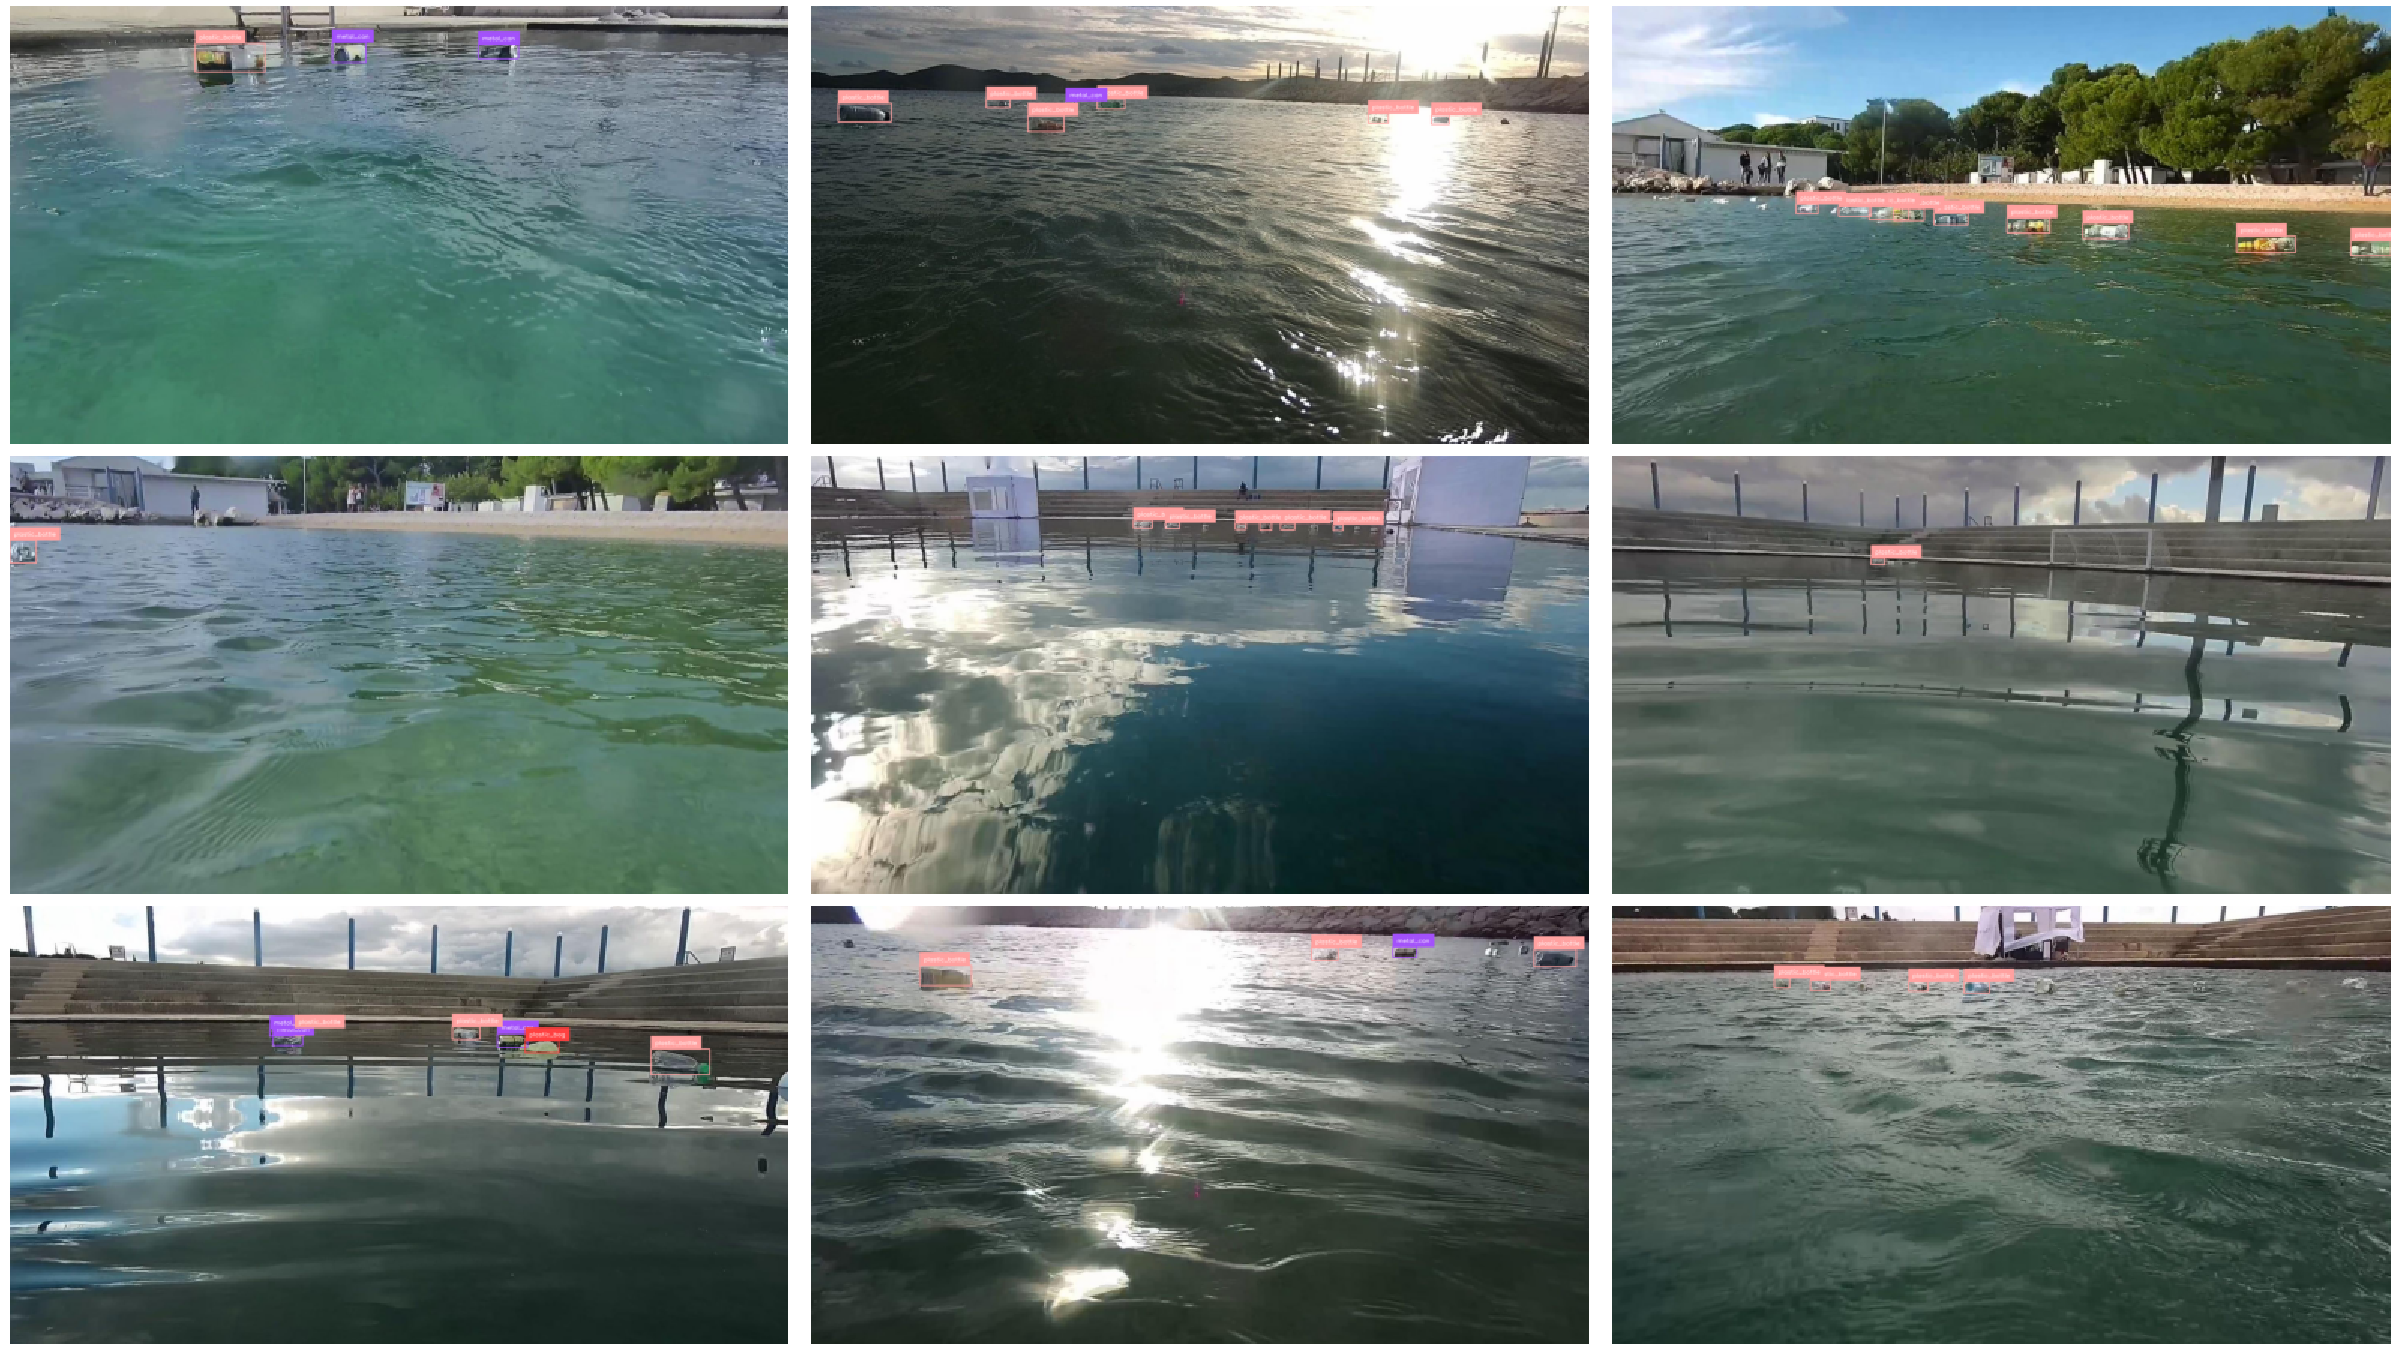
\includegraphics[width=0.86\linewidth,height=5.4cm,keepaspectratio]{figures/sample.pdf}
		\caption{Pink bottle, red bag, purple can. Hikvision PTZ, 1080p.}
		\label{fig:slides-samples}
	\end{figure}
\end{frame}

\begin{frame}{YOLO26 vs RF-DETR}
	\begin{columns}[T]
		\begin{column}{0.47\textwidth}
			\begin{itemize}
				\item YOLO26: local conv, fast~\cite{yolo26_ultralytics}
				      \begin{itemize}
					      \item Nano--XL, 2.3--59M params
				      \end{itemize}
				\item RF-DETR: global attention~\cite{rf-detr}
				      \begin{itemize}
					      \item Nano--XL, 4.1--126M params
				      \end{itemize}
				\item Both COCO SOTA baselines~\cite{lin2015microsoft}
				\item 100 epochs, AdamW, mosaic augmentation
			\end{itemize}
		\end{column}
		\begin{column}{0.49\textwidth}
			\centering
			\begin{tikzpicture}[
					box/.style={thick, rounded corners=2pt, minimum width=2.2cm, minimum height=0.8cm, font=\scriptsize, align=center},
					lab/.style={font=\scriptsize\bfseries},
				]
				\node[lab] (img) at (0, 0) {Sea image};
				\node[box, fill=softgreen!15, draw=softgreen!80!black] (cnn) at (-1.3, -1.2) {YOLO26\\conv stack};
				\node[box, fill=softblue!12, draw=softblue] (att) at (1.3, -1.2) {RF-DETR\\attention};
				\node[lab] (out) at (0, -2.7) {Boxes + labels};
				\draw[-{Stealth}, thick, softgreen!80!black] (img) -- (cnn);
				\draw[-{Stealth}, thick, softblue] (img) -- (att);
				\draw[-{Stealth}, thick, softgreen!80!black] (cnn) -- (out);
				\draw[-{Stealth}, thick, softblue] (att) -- (out);
			\end{tikzpicture}
		\end{column}
	\end{columns}
\end{frame}
